\chapter{Results}\label{chap:results}

We have implemented this method both as standalone and as a~plugin for a~real-time planet renderer as we already mentioned in the~introduction. We did so in order to evaluate the~usability of the~method in practice on real data. With this method used by the~renderer, we compressed and then real-time viewed the~whole-Earth height data with 90m span between height samples (SRTM\footnote{http://www2.jpl.nasa.gov/srtm/}~\cite{srtm}). The~total size of this dataset is 58~GB. Due to the~data redundancy of the~LOD hierarchy of the~renderer which is caused by the~fact that it stores all LODs of terrain completely separately, the~total size of the~SRTM dataset converted to this hierarchy was 260GB. When we applied this compression method to every independent square node of this LOD hierarchy, we managed to compress this data down to 7GB with the~maximum deviation of the~compression set to 5m. This yields the~compression ratio of 37:1. However, if we take the~size of the~original SRTM dataset as the~original size, the~compression ratio will drop to just about 8:1. It needs to be said that the~first ratio is solely the~credit of our method, whereas the~second one is influenced by both the~way the~renderer handles the~data and our method. 

For a~comparison, C-BDAM~\cite{cbdam} achieved the~compression ratio of 64:1 on the~same 90m-resolution SRTM dataset with the~maximum error bound set to 16m. As we already mentioned, C-BDAM contains its own LOD rendering hierarchy without any redundancy --- a~finer LOD is constructed from the~coarser one which is where the~compression takes place. Thanks to this, there is no data redunduncy in the~LOD hierarchy of C-BDAM, so the~compression ratio of this method was evaluated with respect to the~original size of the~dataset which is 58~GB. The~final size of the~compressed data prepared for rendering in C-BDAM was just 870MB.

The~most accurate comparison of our method with C-BDAM we could perform was compress the~SRTM dataset prepared for rendering in the~mentioned application by our method with the~maximum deviation set to 16m. We did so, the~final size of the~data was ???~GB which yield the~compression ratio of ??? when compared to the~size of the~dataset prepared for the~renderer (260~GB) and the~compression ratio of ??? when compared to the~original size of the~dataset (58~GB). Again, the~first compression ratio is only the~credit of our method, whereas the~second one is also influenced by the~way the~data is handled by the~renderer (the~LODs redundancy, overlaps, etc.). However, in terms of functionality, C-BDAM is not analogic to our method, because our method cannot handle the~rendering. It is only analogic to the~renderer with our method plugged in --- only this way, both compression and rendering are achieved. For this reason, the~second compression ratio is the~most relevant one for comparison, even though the~implementation of the~renderer is completely out of the~scope of this thesis. Even though the~compression ratio resulting from the~usage of this renderer together with our method is worse than the~one achieved by C-BDAM, the~redundancy of the~LOD hierarchy of the~renderer has some benefits which have already been mentioned in the~introduction --- mainly much faster access to the~data. Whereas this renderer is able to render a~scene viewed from quite close to the~ground quite quickly because it only needs to fetch the~relevant LODs which are stored indepentendly, this is not the~case of C-BDAM --- to display such a~scene, it needs to gradually reconstruct every ancestor LOD node of the~nodes displayed in the~scene which undoubtedly takes more time. However, we did not measure these times. 

Fig.~\ref{fig:result_samples} shows a~part of a~heightmap compressed by this method, along with the~differences from the~original.

\newcommand{\hspaceimg}{\hspace{0.05cm}}
\newcommand{\vspaceimg}{\vspace{0.15cm}}
\newcommand{\incexamplsolo}[1]{\includegraphics[width=0.5\textwidth]{#1}}

\begin{figure}
	\begin{center}
	\incexamplsolo{figures/samp_orig.png} \\ \vspaceimg
	\incexamplsolo{figures/samp_comp.png} \\ \vspaceimg
	\incexamplsolo{figures/samp_diff.png}
	\end{center}
	\caption{From the~top to the~bottom --- the~original terrain, the~same terrain compressed with the~maximum deviation of 5m, the~difference between these~two. The~brighter the~color, the~greater the~value. In the~difference image, the~yellow color means 4.5m, whereas the~blue color means -4.5m.}
	\label{fig:result_samples}
\end{figure}

\newcommand{\incexamplpair}[1]{\includegraphics[width=0.45\textwidth]{#1}}

\begin{figure}
	\begin{center}
	\incexamplpair{figures/dim_64_amp_16_lon_4_horizontal_orig.png} \hspaceimg
	\incexamplpair{figures/dim_64_amp_16_lon_16_horizontal_orig.png} \\ \vspaceimg
	\incexamplpair{figures/dim_64_amp_16_lon_4_horizontal_out.png} \hspaceimg
	\incexamplpair{figures/dim_64_amp_16_lon_16_horizontal_out.png} \\ \vspaceimg
	\incexamplpair{figures/dim_64_amp_16_lon_4_horizontal_diff.png} \hspaceimg
	\incexamplpair{figures/dim_64_amp_16_lon_16_horizontal_diff.png}
    \end{center}
	\caption{Two synthetic test images of size 64x64, each one containing spiky terrain with the~heights ranging from -16 to 16. On the~left, the~longitude of spikes is 4, on the~right, it is 16. From the~top to the~bottom --- the~original, compressed with the~maximum deviation of 5, the~difference between these~two. The~brighter the~color, the~greater the~value. In the~difference image, the~yellow color means 4.5, whereas the~blue color means -4.5.}
	\label{fig:result_wave_samples}
\end{figure}

\section{The~compression artifacts}\label{sec:artifs}

This section is dedicated to the~artifacts visible in the~terrain compressed by this method. We will explain why they usually occur, analyze what design choice inside the~methods affect their appearance and give some grayscale example visualisations of how they look. We also describe the~modifications to our method with the~help of which we tried to reduce them, but finally did not succeed. Finally, we at least say how they can be reduced in post-processing outside the~method.

Because this method is designed with the~maximum height error as the~only measurement of quality of the~compressed data, we cannot guarantee that the~resulting terrain will look smooth and will not contain any sharp peaks within the~maximum-error bound. Due to the~character of the~method, such artifacts indeed occur and we have not found out how to modify the~method, so that they can be avoided. However, at least we reduced them by choosing the~most suitable prediction operator $\opnorm{P}{b}$ and $\opnorm{P}{c}$ --- Neville interpolating filter of order 2 --- for all pixels, both near the~mip-map edges and in its interior.

As we already said in Section~\ref{sec:top-down}, C-BDAM only uses the~order 2 filter for the~pixels near the~borders and the~order 4 filter for the~rest of them. We tried using the~order 4 filter with various weights settings for the~interior values, too. This slightly increased the~compression ratio --- probably because this~filter is better at predicting hills and valleys --- but worsened the~quality of compression by producing more significant artifacts. We have found some general situations in which they are particularly disturbing --- near smooth terrain's borders (Fig.~\ref{fig:artifs_border}) and near sharp terrain transitions (Fig.~\ref{fig:artifs_sharp_change}). The~most probable cause of this is that the~predictions made by the~order 4 filter tend to differ from the~neighboring heights more. This emphasises the~artifacts.

\newcommand{\vcentered}[1]{\begingroup\setbox0=\hbox{#1}\parbox{\wd0}{\box0}\endgroup}

\newcommand{\artifWidth}{160}
\newcommand{\artifHeight}{120}
\newcommand{\incimg}[3]{\includegraphics[width=#1px, height=#2px]{#3}}
\newcommand{\incimgvcenter}[3]{\vcentered{\incimg{#1}{#2}{#3}}}
\newcommand{\incartifborder}[1]{\incimgvcenter{\artifWidth}{\artifHeight}{#1}}
\newcommand{\hspacehead}{\hspace{0.4cm}}

\begin{figure}
	\begin{center}
	Original\hspacehead\incartifborder{figures/artif_orig0.png} \hspaceimg
	\incartifborder{figures/artif_orig1.png} \\ \vspaceimg 
	Order 2\hspacehead\incartifborder{figures/artif_four0.png} \hspaceimg
	\incartifborder{figures/artif_four1.png} \\ \vspaceimg
	Order 4\hspacehead\incartifborder{figures/artif_twelve0.png} \hspaceimg
	\incartifborder{figures/artif_twelve1.png} \\ \vspaceimg
	\end{center}
	\caption{Two examples of the~difference between artifacts caused by order 2 and order 4 filters near smooth terrain's border --- in the~first row there are the~target heightmaps, in the~second, there are the~same heightmaps compressed using the~order 2 filter, in the~third row, the~heightmaps compressed with the~order 4 filter.}
	\label{fig:artifs_border}
\end{figure}

\newcommand{\incartifchange}[1]{\incimgvcenter{\artifWidth}{\artifWidth}{#1}}

\begin{figure}
	\begin{center}
	Original\hspacehead\incartifchange{figures/artif_change_orig0.png} \hspaceimg
	\incartifchange{figures/artif_change_orig1.png} \\ \vspaceimg
	Order 2\hspacehead\incartifchange{figures/artif_change_four0.png} \hspaceimg
	\incartifchange{figures/artif_change_four1.png} \\ \vspaceimg
	Order 4\hspacehead\incartifchange{figures/artif_change_twelve0.png} \hspaceimg
	\incartifchange{figures/artif_change_twelve1.png} \\ \vspaceimg
	\end{center}
	\caption{Two examples of the~difference between artifacts caused by order 2 and order 4 filters near a~sharp terrain change --- in the~first row there are the~target heightmaps, in the~second row, the~same heightmaps compressed using the~order 2 filter, in the~third row, the~heightmaps compressed with the~order 4 filter. The~span of the~values in the~original images is from 0 to 16 and the~maximum absolute deviation ($D$) of compression is set to 9.}
	\label{fig:artifs_sharp_change}
\end{figure}

Generally, the~reason why these artifacts occur is that as long as the~predictions are close enough to the~target mip-map and their quantized residuals are equal to zero, the~compressed values might remain above/under the~terrain for a~long time, but only until one prediction gets a~bit further from the~target terrain. As soon as it happens, its associated residual will be quantized to a~certain non-zero value which will result in the~reconstructed value being flipped to the~opposite side of the~real terrain which produces a~visual artifact. It is not a~coincidence that this often occurs near a~sharp change in the~terrain. The~predictions produced by the~averaging filter get a~bit different from the~adjacent ones near this change, because at these places, the~filter reaches out to the~area behind the~change (Fig.~\ref{fig:artifs_theory}). This difference might then cause the difference in residuals --- the~quantized residuals further from this change might be all zeroes, whereas the~residual near this change not, causing a~spike to occur. This spike will then get propagated to the~following compressed mip-map levels. The~only thing that is guaranteed is that the~maximum error bound is still satisfied. The~clipping performed by the~predicting filter near the~mip-map borders creates the~effect similar to a~sharp terrain change, too, in a~bit different way --- by the~sole fact that the~terrain behind the~border no longer follows its trend up to the~border (rising, for example), but is practically mirrored behind the~border (following the~example, falling), because instead of reaching out to the~non-existing values out of the~mip-map, the~existing ones are used.

\begin{figure}
	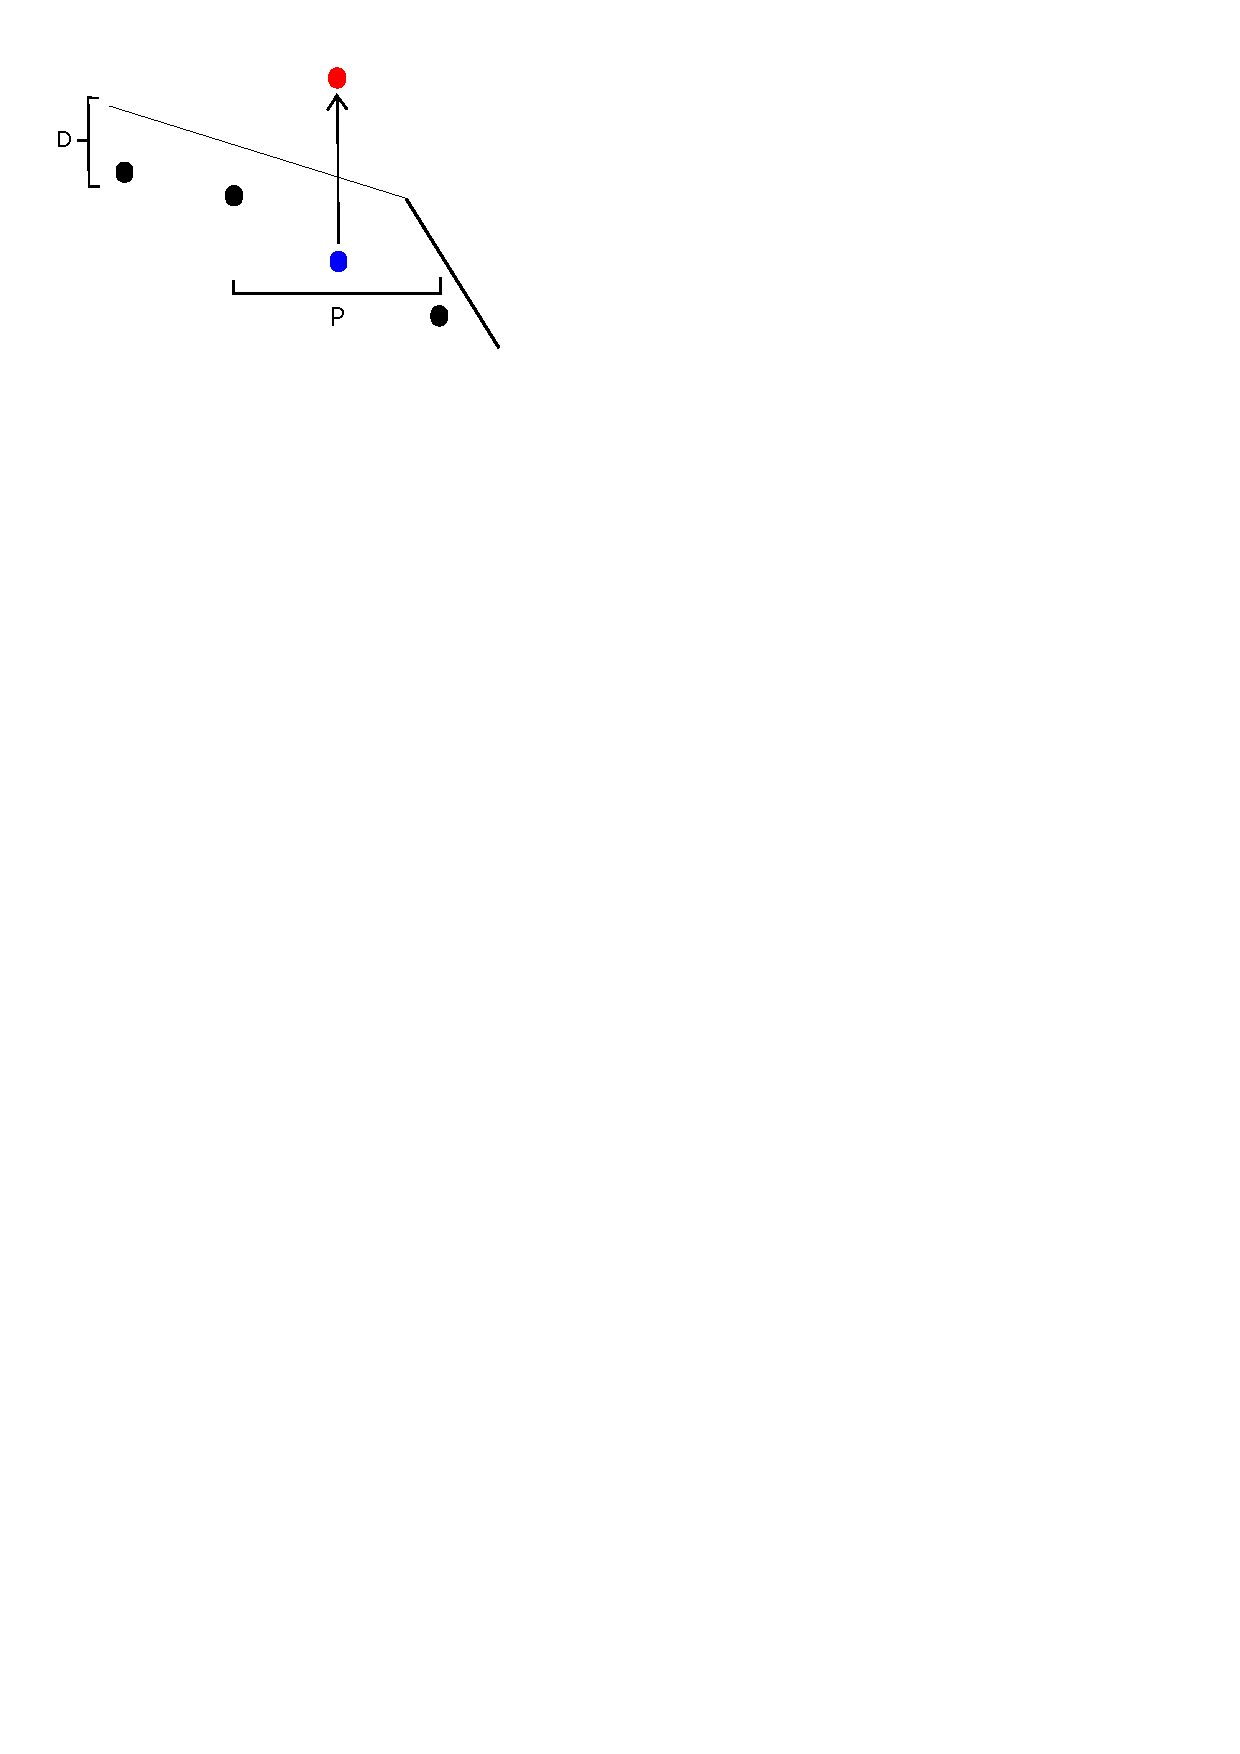
\includegraphics[trim={0 24cm 13cm 1cm}, clip, width=0.45\textwidth]{figures/artifs_theory.pdf}\centering
	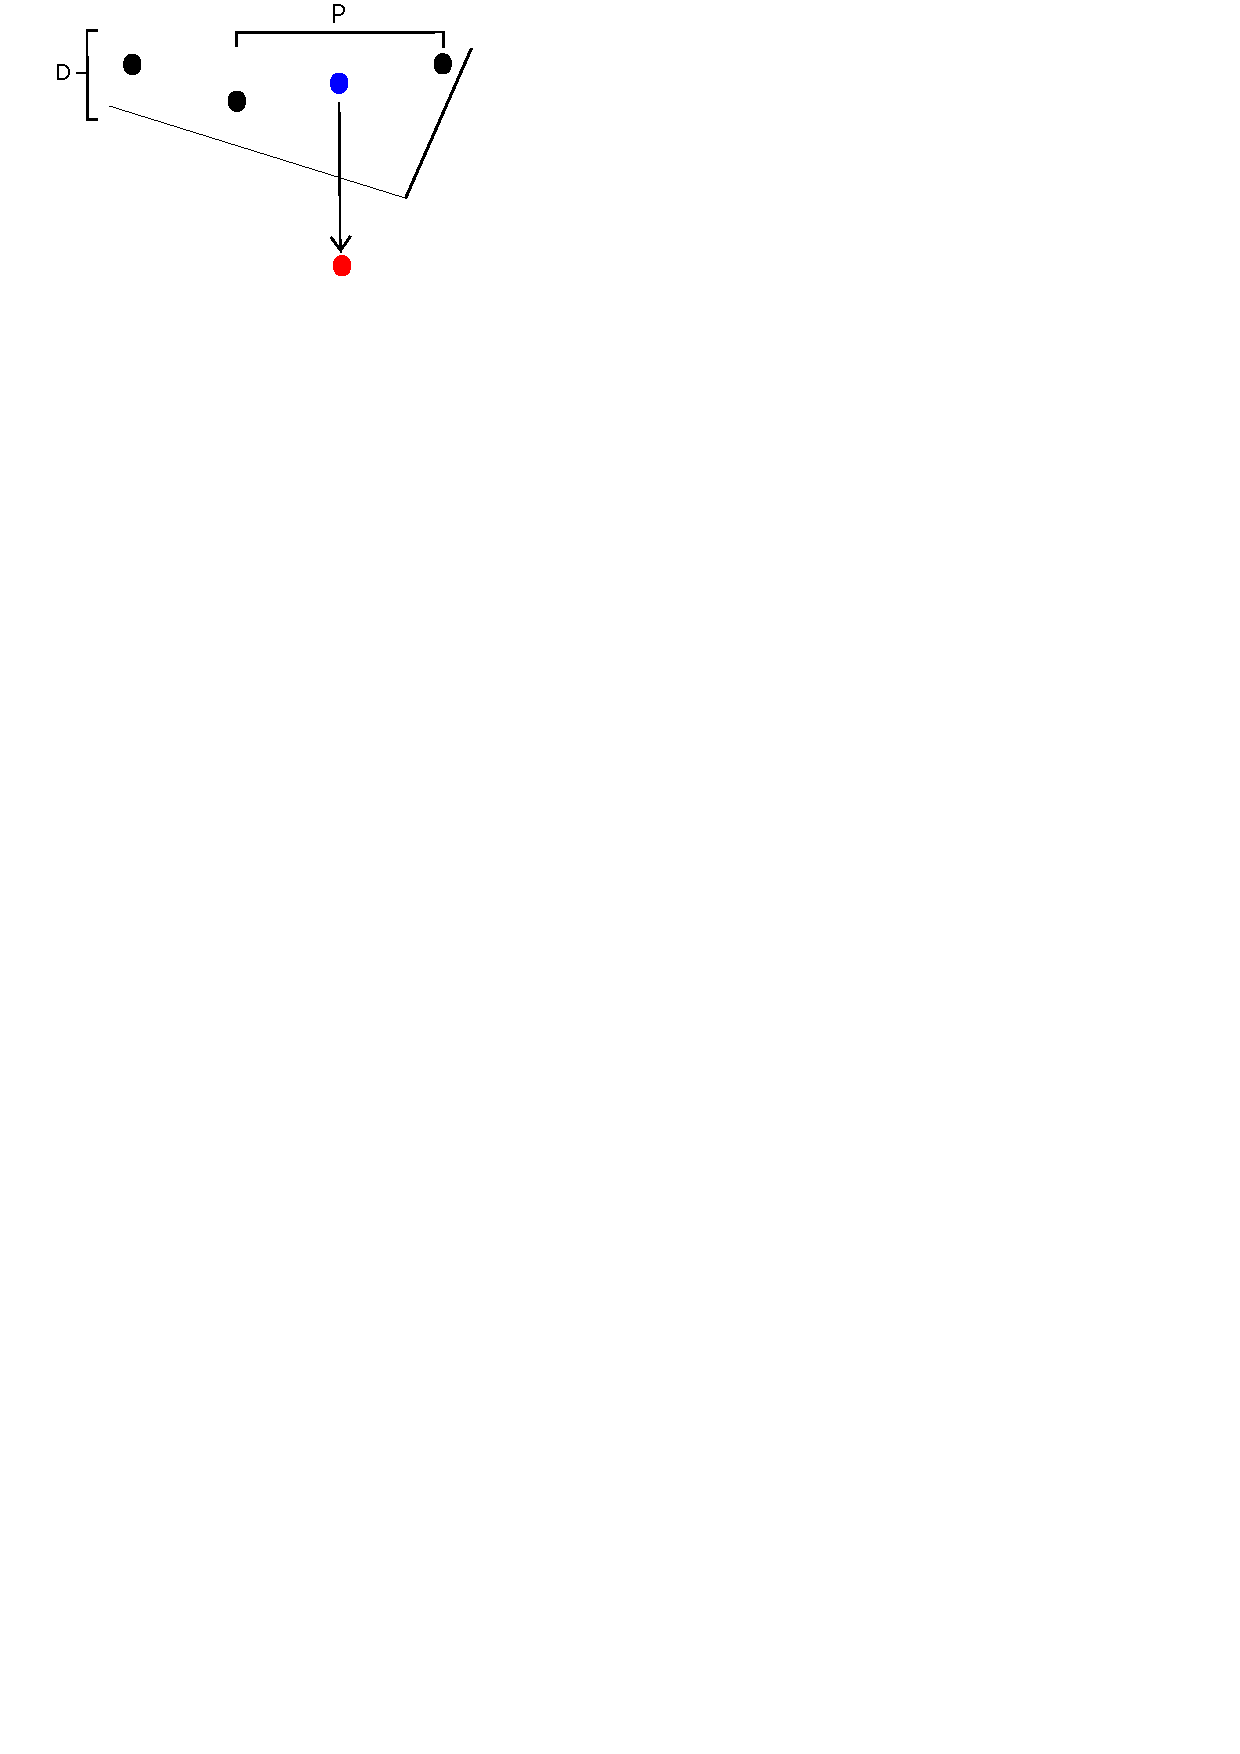
\includegraphics[trim={0 24cm 13cm 0}, clip, width=0.45\textwidth]{figures/artifs_theory2.pdf}\centering
	\caption{Two illustrations of how artifacts can occur near sharp terrain changes --- the~black dots stand for the~predictions which are still within the~maximum-error bound $D$ from the~target terrain, the~blue dots represent the~predictions which are just slightly further from the~terrain, because their filters span to the~area behind the~change. Due to the~fact that a~uniform quantizer with the~step of $2D-1$ is applied to the~residuals, the~residuals added to the~blue predictions will cause them to be shifted by $2D - 1$ to the~top (the~image on the~left) or to the~bottom (the~image on the~right), creating sharp peaks in the~reconstructed values --- the~artifacts.}
	\label{fig:artifs_theory}
\end{figure}

We also tried to apply progressive quantization to the~residuals in order to try to reduce the~ artifacts in the~reconstructed terrain. In Sec.~\ref{sec:wavelets}, we mentioned that progressive quantization degrades the~coarser residuals less than the~finer (more detailed) ones. In our context, it would mean that the~maximum error of $\objdot{L}{i}$ (the~reconstructed data) equal to the~quantization interval of $\objdot{E}{i}$ (the~quantized residuals) would grow with $i$ up to $D$ at the~finest level. However, more careful decimation of coarser high-pass information only helps reduce large-scale artifacts which is not the~case of our artifacts --- they are mainly caused by differences between neighboring pixels which happens due to the~fact that the~residuals are cropped to respect the~maximum deviation. Indeed, our experiments with progressive quantization did not help reduce the~artifacts at all --- progressive quantization does not tackle the~problem described in the~previous paragraph.